\section{STT-RAM Macro Modeling} \label{sec:model}
Some modeling issues will be discussed in this section.

\subsection{Area Modeling}
To simulate the performance of a single STT-RAM cell, it is important to estimate its access area first. As mentioned before, each 1T1J STT-RAM cell is composed of one NMOS and one MTJ. The NMOS access device is connected in series with the MTJ as shown in Figure~\ref{fig:1t1r}. The size of NMOS is constrained by both $I_{c}(AP\rightarrow P)$ and $I_{c}(P\rightarrow AP)$, which are inversely proportional to the writing pulse width. In order to estimate the current driving ability of MOSFET devices, a small test circuit using HSPICE with PTM 45nm HP model~\cite{PTM} is simulated. The BL-to-SL current and SL-to-BL current are obtained by assuming typical TMR (120\%) and LRS ($3k\Omega$) value~\cite{STTRAM:Qualcomm09} and bursting wordline voltage to be 1.5V (the optimal $V_{WL}$ value is extracted from~\cite{STTRAM:Gatech10}). As we can see in Figure~\ref{fig:hspice}(a), the SL-to-BL current is always smaller and saturate faster than BL-to-SL current. Such current degradation is related to the body effect of the access transistor, where the threshold voltage is boosted by a positive source-to-substrate voltage different $V_{SB}=I_{c}\times R$ ($I_{c}$ is the current passing through MTJ and $R$ is the resistance of the MTJ). Thus we always choose the connecting scheme which use BL-to-SL current to match the maximum of $I_{c}(AP\rightarrow P)$ and $I_{c}(P\rightarrow AP)$ and SL-to-BL to match the minimum of them. The corresponding access transistor width must satisfy the following conditions,
\begin{eqnarray}
I_{BS}(W_{BS}) &\geq& max(I_{c}(AP\rightarrow P), I_{c}(P\rightarrow AP)) \\
I_{SB}(W_{SB}) &\geq& min(I_{c}(AP\rightarrow P), I_{c}(P\rightarrow AP))
\end{eqnarray}
where $I_{BS}(W_{BS})$ is the current from BL to SL with transistor width $W_{BS}$ and $I_{SB}(W_{SB})$ is the current from SL to BL with transistor width $W_{SB}$.

\begin{figure}[t]
  \centering
  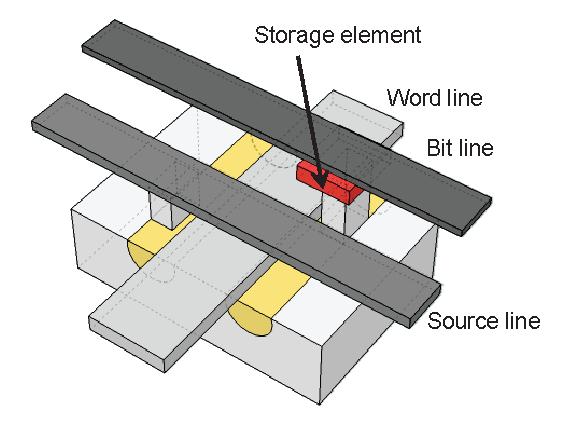
\includegraphics[width=2.5in]{fig/1t1r.eps}
  \vspace{-10pt}
  \caption{Conceptual view of a MOS-accessed cell (1T1J) and its connected word line, bit line, and source line.}
  \label{fig:1t1r}
  \vspace{-5pt}
\end{figure}

\begin{figure}[t]
  \centering
  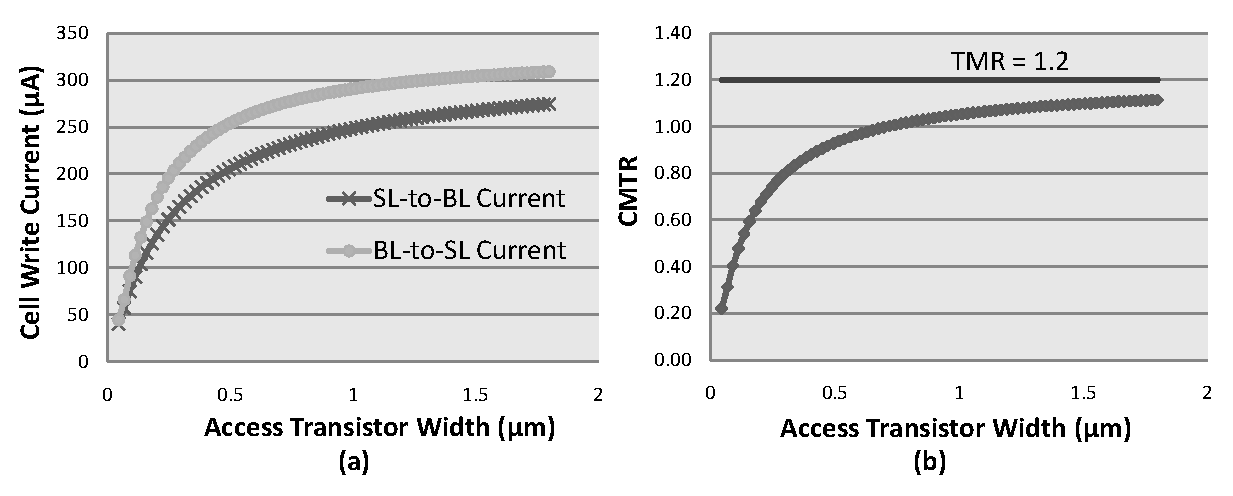
\includegraphics[width=3.5in]{fig/HSPICE.eps}
%  \vspace{-10pt}
  \caption{(a) Driving ability, and (b) Cell TMR of access NMOS transistor.}
  \label{fig:hspice}
  \vspace{-15pt}
\end{figure}

The relationship between access transistor width and CTMR defined in Section~\ref{subsec:cell} was also simulated. As can be seen in Figure~{fig:hspice}(b), a larger access transistor increase CTRM closer to the inherent TRM value of MTJ. It's necessary to set a lower bound $CTMR_{min}$ for CTMR to guarantee the correctness of read operation. Thus the transistor width must be large enough to satisfy the minimum CTMR requirement,
\begin{equation}
CTMR(W_{CTMR}) \geq CTMR_{min}
\end{equation}
Finally we will choose a transistor width $W$ which satisfy all the above requirements,
\begin{equation}
W = max(W_{BS}, W_{SB}, W_{CTMR}) \label{equ:width}
\end{equation}

To achieve high cell density, we model the STT-RAM cell area by referring to DRAM design rules~\cite{DRAM:6F2}.  As a result, the cell size of a STT-RAM cell is calculated as follows,
\begin{equation}
\mathrm{Area}_{\mathrm{cell}}={3\left(W/L+1\right)}(F^2)
\end{equation}

\subsection{Data sensing modeling}
Three sensing modes were proposed in~\cite{CACTI:DATE11:Xu} to sense resistance-based NVMs including STT-RAM, PCRAM and ReRAM: current sensing, current-in voltage sensing, and voltage-divider sensing. There are trade-offs between the area, latency and energy of the three sensing modes. For example, current sensing is the fastest approach~\cite{RRAM:ITRI11} to sense the state if the number of cells per bitline is larger than 64, while voltage-divider sensing the second fastest and the current-in voltage sensing is slowest. In contrast, current-in voltage sensing has the best area efficiency which is defined as the ratio of NVM cell area to the prototype area while current-in sensing has the worst area efficiency. In this work, we will focus on current sensing scheme to reduce read latency. We adapt the current-voltage converter and sense amplifier design discussed in~\cite{CACTI:DAC08:Dong}. The current-voltage converter in our current sensing scheme is actually the first-level sense amplifier, and the conventional voltage sense amplifier is still kept as the final stage of the sensing scheme. In order to maintain low rate of read disturbance, it's necessary to reduce read current when choosing longer write pulse and smaller write current. And reduced read current have impact on the latency of current-voltage converter and sense amplifier. Therefore We use HSPICE to simulate the latency, energy and leakage of the two-stage sense amplifier with different read current and build a look-up table in NVsim.

\subsection{Cell Switching Modeling} \label{subsec:co-opt}
Dynamic MTJ switching model was developed in~\cite{STTRAM:Purdue10} with consideration of the switching phenomenon involves magnetoresistive effects, which can not estimated only by RC analysis.  However, this work is focusing on static analysis of STT-RAM and NVSim does not model the dynamic behavior during the switching of the cell state. Thus we use simply calculate switching energy (i.e. cell write energy) by using Joule's first law that is,
\begin{equation}
\mathrm{Energy}_{\mathrm{cell\_switching}} = I_{c}^2 R \tau \label{equ:cellenergy}
\end{equation}
in which the resistance value $R$ can be the equivalent resistance of the corresponding LRS or HRS (i.e. $R_{P}$ or $R_{AP}$). Taking the switching current versus switching pulse width as input for Equation~\ref{equ:cellenergy}, we can easily get the relation between the energy of switching one cell and write pulse width. It can been seen in Figure~\ref{fig:cellenergy}, minimum switching energy per cell is achieved at write pulse width $\tau_{min\_cell\_energy}$ in the range of processional switching mode. However, the the optimal operating write pulse width from cell-level point of view is not necessarily the best operating point from system-level point of view because the effect of access transistor and peripheral circuitry have not been considered.
\begin{figure}[t]
  \centering
  \includegraphics[width=2.5in]{fig/cellenergy.eps}
  \vspace{-10pt}
  \caption{Switching energy per cell versus write pulse width.}
  \label{fig:cellenergy}
%  \vspace{-15pt}
\end{figure}

